%%%%%%%%%%%%%%%%%%%%%%%%%%%%%%%%%%%%%%%%%%%%%%%%%%%%%
%			    Generic Slave module				%
%					-----------						%
% Author: Thibault Porteboeuf						%
%%%%%%%%%%%%%%%%%%%%%%%%%%%%%%%%%%%%%%%%%%%%%%%%%%%%%

\section{Generic Slave Module}

As several modules in our design require a slave interface to let the LM32 post to them configuration values, we decided to implement a generic slave interface, that can be easily re-used in every module.

This generic slave modules includes a state machine that handles simple read and write requests, as presented in figure \ref{state_machine_slave}.

\begin{figure}[h]
\center
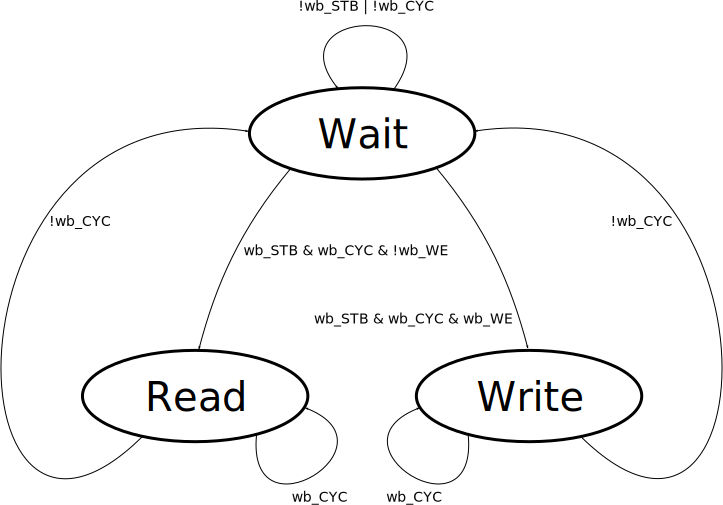
\includegraphics[width=11cm]{figs/slave_state_machine.pdf}
\caption{Generic slave's state machine}
\label{state_machine_slave}
\end{figure}

When accessing the \emph{Read} or \emph{Write} states, the module automatically calls the \texttt{slave\_read()} and \texttt{slave\_write()} methods respectively.

These methods can be overloaded in any inheriting slave interface, and thus allows a great variety of behaviors and features to rely on one single wishbone slave interface.
